\documentclass[11pt]{article}
\usepackage[margin=1in]{geometry}
\usepackage{graphicx}
\usepackage{amsmath}
\usepackage{amssymb}
\usepackage{hyperref}

\title{Assignment 3: Mandelbrot Set and Lorenz System}
\author{Elena Osipyan}
\date{}

\begin{document}

\maketitle
\vspace{-1cm}

\section{Question 1: The Mandelbrot Set}

 For each point in the complex plane $c = x + iy$, I iterated the map $z_{i+1} = z_i^2 + c$, starting from $z_0 = 0$. The goal was to see whether the iterates remain bounded or diverge to infinity. I divided the complex plane on a grid with $-2 < x < 2$ and $-2 < y < 2$, dividing each dimension into 100 equally spaced points. For each point $c$, I computed the iteration at which $|z| > 2$, using a maximum of 30 iterations. This threshold was chosen because iterates with magnitude exceeding 2 are guaranteed to diverge to infinity.

The core iteration logic is in a separate Python module (\texttt{comp\_calc.py}). The iteration function returns either the iteration number at which divergence occurs, or the maximum iteration count for bounded points.

Figure \ref{fig:mandelbrot1} displays the classification of points as bounded (Mandelbrot set members) versus diverged points.  Figure \ref{fig:mandelbrot2}  colors each point by the iteration number at which it diverges. The figures resemble the shape of the Mandelbrot set \cite{mandelbrot1980}. When looking at the iteration counts, which show rapid transitions between bounded and unbounded regions, we can see that it is a fractal.

\begin{figure}[h]
\begin{center}
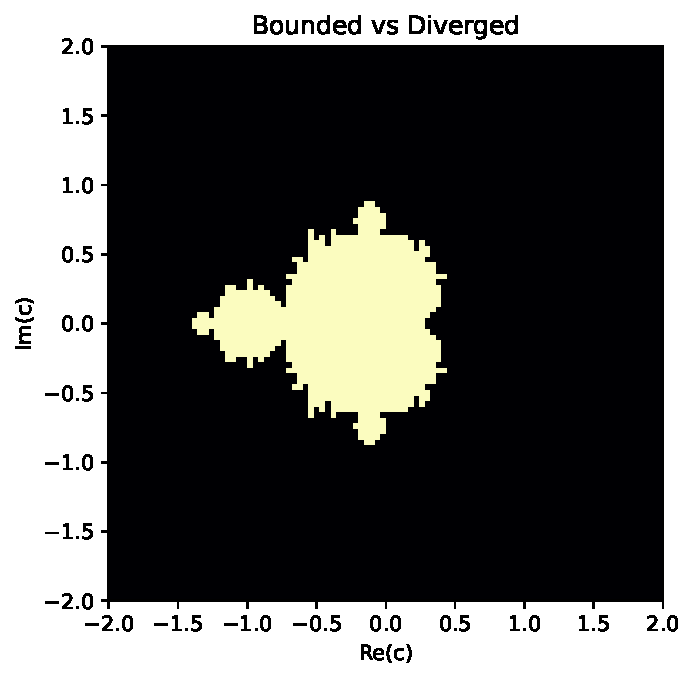
\includegraphics[width=0.4\linewidth]{mandelbrot_bounded}
\caption{Classification of points in the complex plane as bounded (white) or diverged (black). The Mandelbrot set is clearly visible as the white region.}
\label{fig:mandelbrot1}
\end{center}
\end{figure}

\begin{figure}[h]
\centering
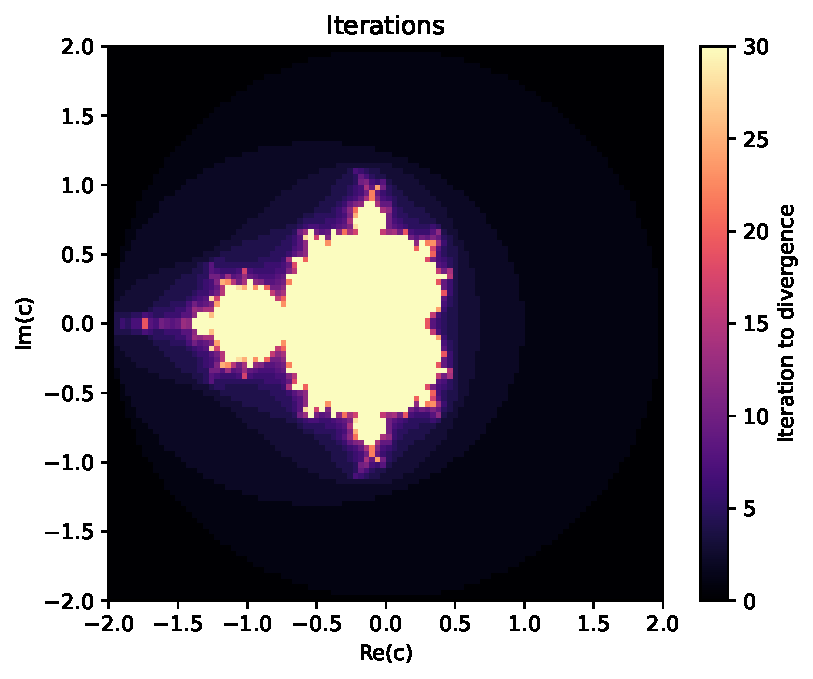
\includegraphics[width=0.6\textwidth]{mandelbrot_iterations.pdf}
\caption{Points colored by iteration number at which they diverge. The color scale ranges from 0 to 30 iterations, revealing the fractal boundary structure of the Mandelbrot set.}
\label{fig:mandelbrot2}
\end{figure}

\newpage

\section{Question 2}

\subsection{Mathematical Framework and Implementation}

Lorenz's system consists of three coupled nonlinear ordinary differential equations, where $\sigma = 10$ is the Prandtl number (ratio of kinematic viscosity to thermal diffusivity), $r = 28$ is the Rayleigh number (related to the temperature difference driving convection), and $b = 8/3$ is a dimensionless length scale. The initial conditions are $W_0 = (X_0, Y_0, Z_0) = (0, 1, 0)$ \cite{lorenz1963}.

I integrated these equations using the Runge-Kutta 45 method (\texttt{solve\_ivp} with \texttt{RK45}), chosen for its fifth-order accuracy and adaptive step-size control. The integration time span was $t = 0$ to $t = 60$ dimensionless time units, with output sampled at 6000 equally spaced points (matching Lorenz's original resolution of $\Delta t = 0.01$). The tight coupling of the equations necessitated a maximum step size of 0.01 to ensure numerical stability.

\subsection{Phase Space Dynamics and Attractors}

The first indicator of the system's complex behavior appears in Figure \ref{fig:lorenz_timeseries}, which shows the $Y$-coordinate as a function of iteration count over the first 3000 iterations. These oscillations show irregular amplitude and frequency modulation (chaotic motion).

Figures \ref{fig:lorenz_phase_yz} and \ref{fig:lorenz_phase_xy} present projections of the full three-dimensional phase space trajectory onto the $YZ$ and $XY$ planes respectively. The motion is perfectly deterministic, yet appears random and is highly sensitive to initial conditions.

The two lobes of the attractor correspond to states with different dominant convection patterns. The trajectory spirals outward from one lobe, then jumps unpredictably to spiral around the other lobe. 

\subsection{Sensitive Dependence and Lyapunov Exponents}

The sensitivity analysis is shown in Figure \ref{fig:lorenz_divergence}. I integrated the system with initial conditions $W_0' = (0, 1.00000001, 0)$, differing from the original by only $10^{-8}$ in the $Y$ component. Over time, this small  perturbation grows exponentially. The semilog plot shows the exponential growth of the separation distance between the two trajectories over the first $\sim 20-40$ time units.

This exponential divergence characterizes the Lyapunov exponent, which is a quantitative measure of chaotic behavior. For a system with a positive Lyapunov exponent $\lambda > 0$, nearby trajectories separate as $\delta(t) \approx \delta_0 e^{\lambda t}$. The near-linear behavior in the semilog plot confirms this exponential growth, indicating that the Lorenz system at these parameters is indeed chaotic. Hence, long-term weather prediction is fundamentally limited. Initial uncertainties inevitably affect atmospheric changes.

\begin{figure}[h]
\centering
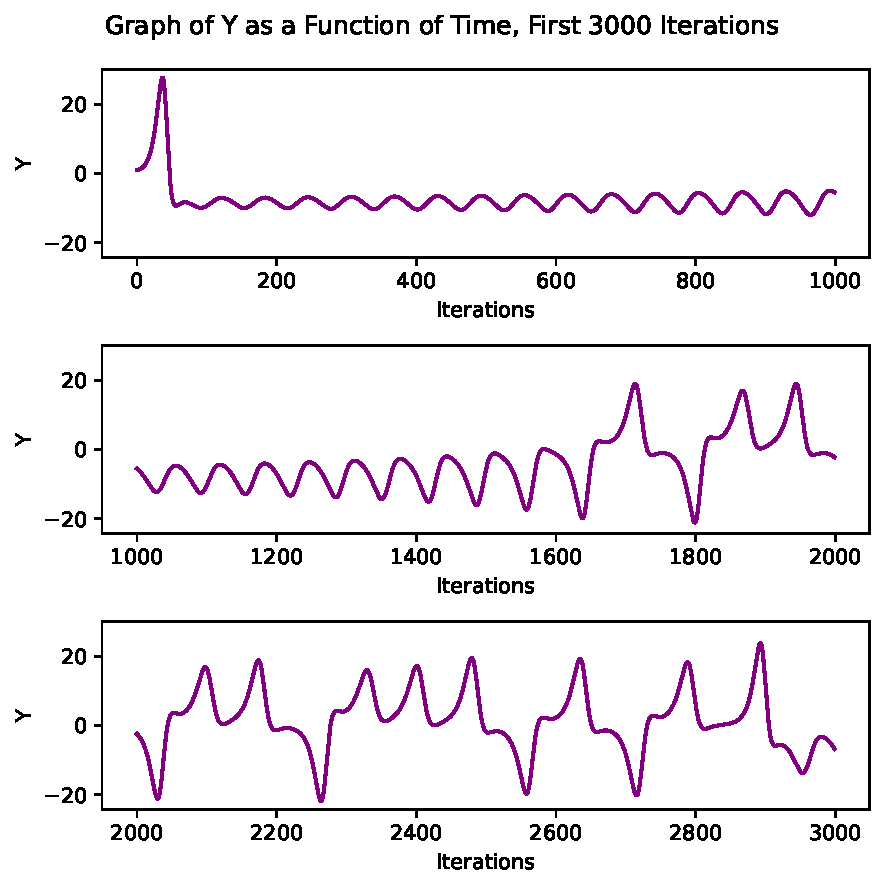
\includegraphics[width=0.6\textwidth]{lorenz_timeseries.pdf}
\caption{Time series of the $Y$ coordinate over the first 3000 iterations. The irregular oscillations with varying amplitude are characteristic of chaotic motion.}
\label{fig:lorenz_timeseries}
\end{figure}
\newpage
\begin{figure}[h]
\centering
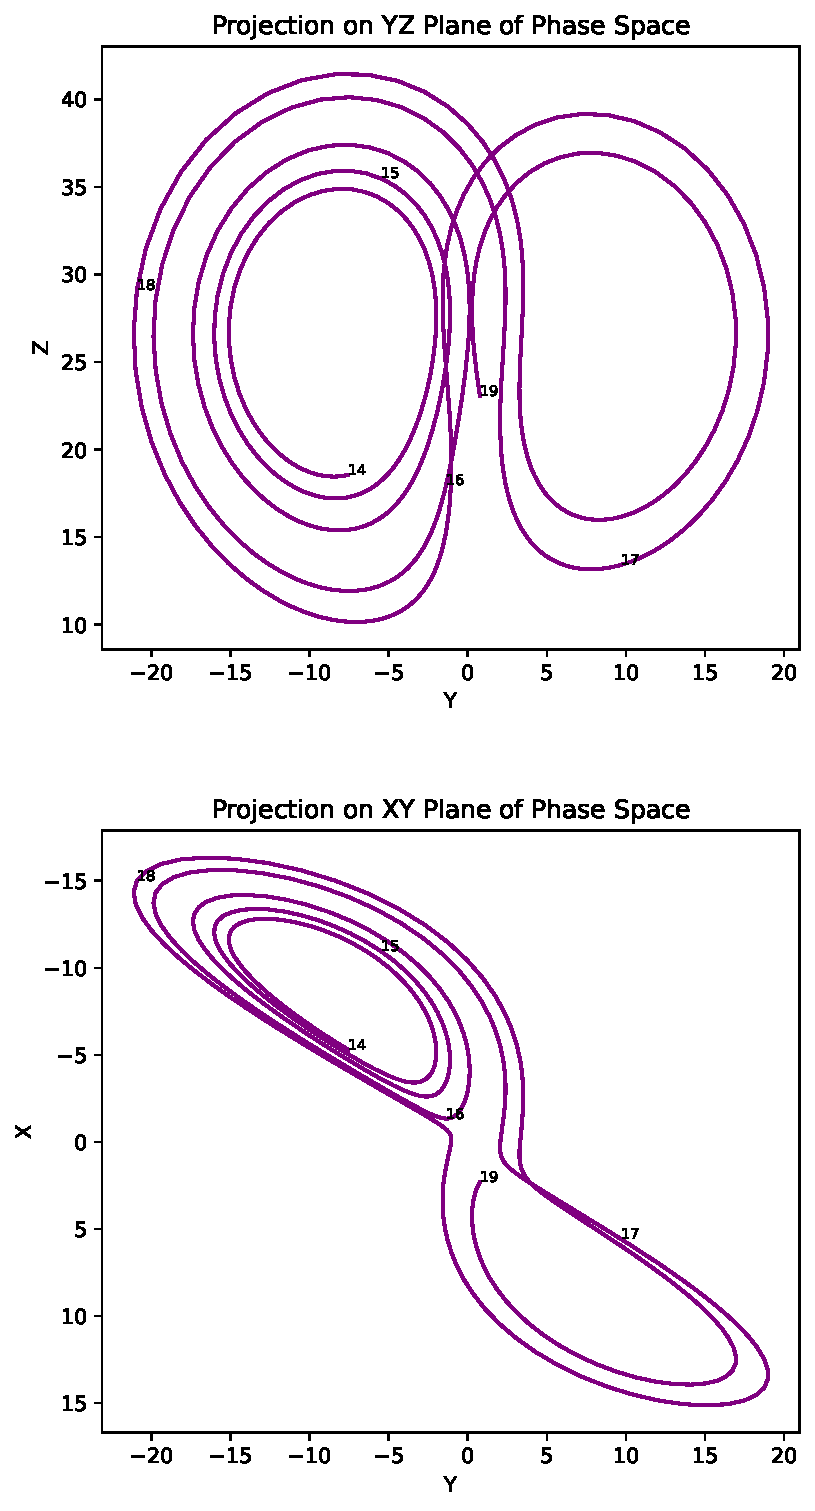
\includegraphics[width=0.6\textwidth]{lorenz_phase_yz.pdf}
\caption{Projection of the Lorenz attractor onto the $YZ$ plane. The two lobes of the strange attractor are clearly visible, showing the complex structure visited by the trajectory.}
\label{fig:lorenz_phase_yz}
\end{figure}

\begin{figure}[h]
\centering
\includegraphics[width=0.6\textwidth]{lorenz_phase_xy.pdf}
\caption{Projection of the Lorenz attractor onto the $XY$ plane. The characteristic butterfly-like shape emerges from this perspective, illustrating why this structure is sometimes called the ``butterfly attractor.'' Numbers mark iterations at 100-step intervals.}
\label{fig:lorenz_phase_xy}
\end{figure}

\begin{figure}[h]
\centering
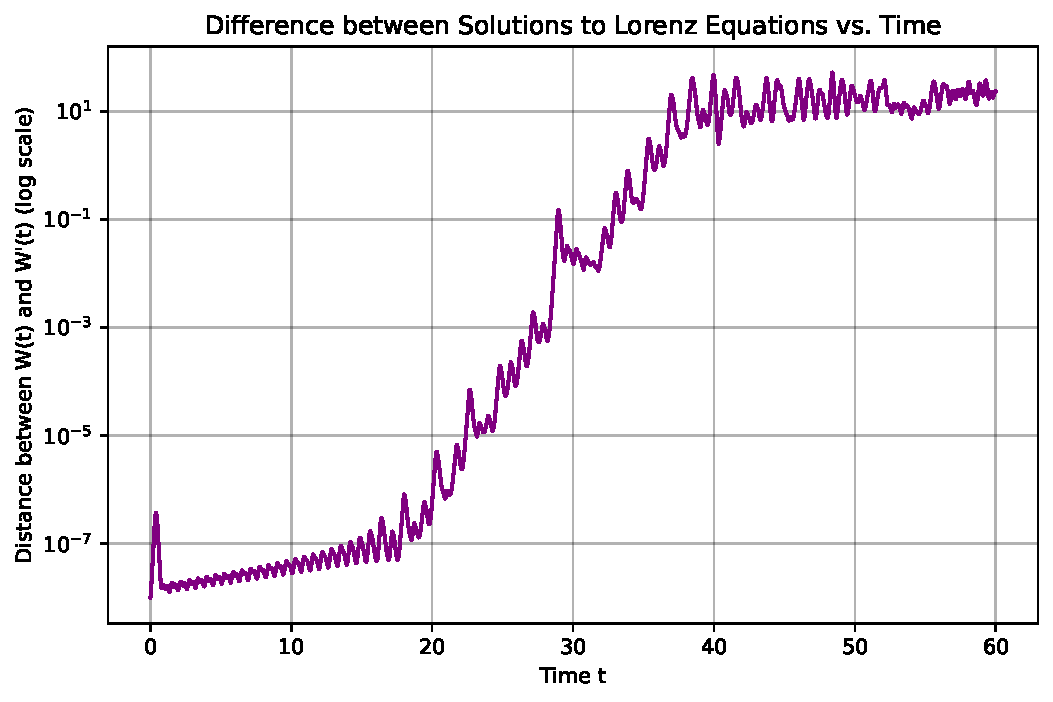
\includegraphics[width=0.6\textwidth]{lorenz_divergence.pdf}
\caption{Exponential divergence of the two trajectories. Small perturbations ($\sim 10^{-8}$) grow exponentially with a Lyapunov timescale of approximately 2.5 time units. After $t \approx 30$, the trajectories stop correlating.}
\label{fig:lorenz_divergence}
\end{figure}
\clearpage

\begin{thebibliography}{99}

\bibitem{mandelbrot1980} Mandelbrot, B. B. (1983). The Fractal Geometry of Nature. \textit{W.H. Freeman and Company}.

\bibitem{lorenz1963} Lorenz, E. N. (1963). Deterministic Nonperiodic Flow. \textit{Journal of the Atmospheric Sciences}, \textbf{20}(2), 130--141. \url{https://journals.ametsoc.org/view/journals/atsc/20/2/1520-0469_1963_020_0130_dnf_2_0_co_2.xml}

\end{thebibliography}

\end{document}
